\documentclass[a4paper,12pt]{article}
\usepackage[unicode,verbose]{hyperref}
\usepackage{amsmath,amssymb,amsthm} \usepackage{pb-diagram}
\usepackage{ucs}
%\usepackage[utf8x]{inputenc}
%\usepackage[russian]{babel}
\usepackage{cmap}
\usepackage[pdftex]{graphicx}
\pagestyle{plain}
\theoremstyle{definition} \newtheorem{Def}{Definition}

%%%%%%%%%%%%%%% From Walton's paper
\def\Z{\Bbb Z}\def\R{\Bbb R}\def\C{\Bbb C}\def\N{\Bbb N}\def\Q{\Bbb Q}
%
\def\la{{\lambda}}\def\al{{\alpha}}\def\be{{\beta}}\def\ga{{\gamma}}
\def\ka{{\kappa}}\def\ome{{\omega}}\def\vp{{\varphi}}
%
\def\Tr{{\rm Tr}\,}\def\ad{{\rm ad}\,}\def\dim{{\rm dim}\,}\def\id{{\rm id}}
\def\ch{{\rm ch}}\def\mult{{\rm mult}\,}
\def\Ppkb{\overline{P_+^k}}
%
\def\zb{{\bar z}}
\def\pzp{{\{z\}}}
\def\di{{\partial}}
\def\h{\hat}
\def\>{{\rangle}}
\def\<{{\langle}}
\def\K{{\cal K}}
\def\T{{\cal T}}
\def\Tn{{\cal T}_\#}
\def\Nk{{{ }^{(k)}N}}\def\Vk{{{ }^{(k)}V}}
\def\Sk{{S^{(k)}}}\def\Tk{{T^{(k)}}}
\def\LR{{Littlewood-Richardson}}
\def\ie{{\rm i.e.}}\def\card{{\rm card}\,}
\def\Sp{{\rm Span}\,}

% standard tableaux
\def\b#1{\kern-0.25pt\vbox{\hrule height 0.2pt\hbox{\vrule
width 0.2pt \kern2pt\vbox{\kern2pt \hbox{#1}\kern2pt}\kern2pt\vrule
width 0.2pt}\hrule height 0.2pt}}
\def\ST#1{\matrix{\vbox{#1}}}
\def\STrow#1{\hbox{#1}\kern-1.35pt}
\def\bv{\b{\phantom{1}}}

\font\huge=cmr10 scaled \magstep2
\font\small=cmr8

% usage: surround part of equation to be boxed by \boxEq{...}
\def\boxit#1{\leavevmode\kern5pt\hbox{
	\vrule width.2pt\vtop{\vbox{\hrule height.2pt\kern5pt
        \hbox{\kern5pt{#1}\kern5pt}}
      \kern5pt\hrule height.2pt}\vrule width.2pt}\kern5pt}
\def\boxEq#1{\boxit{$\displaystyle #1$}}

% Wick contraction (upper-bracket)
\def\ubrackfill#1{$\mathsurround=0pt
	\kern2.5pt\vrule depth#1\leaders\hrule\hfill\vrule depth#1\kern2.5pt$}
\def\contract#1{\mathop{\vbox{\ialign{##\crcr\noalign{\kern3pt}
	\ubrackfill{3pt}\crcr\noalign{\kern3pt\nointerlineskip}
	$\hfil\displaystyle{#1}\hfil$\crcr}}}\limits
}

\def\ubrack#1{$\mathsurround=0pt
	\vrule depth#1\leaders\hrule\hfill\vrule depth#1$}
\def\dbrack#1{$\mathsurround=0pt
	\vrule height#1\leaders\hrule\hfill\vrule height#1$}
\def\ucontract#1#2{\mathop{\vbox{\ialign{##\crcr\noalign{\kern 4pt}
	\ubrack{#2}\crcr\noalign{\kern 4pt\nointerlineskip}
	$\hskip #1\relax$\crcr}}}\limits
}
\def\dcontract#1#2{\mathop{\vbox{\ialign{##\crcr
	$\hskip #1\relax$\crcr\noalign{\kern0pt}
	\dbrack{#2}\crcr\noalign{\kern0pt\nointerlineskip}
	}}}\limits
}

\def\ucont#1#2#3{^{\kern-#3\ucontract{#1}{#2}\kern #3\kern-#1}}
\def\dcont#1#2#3{_{\kern-#3\dcontract{#1}{#2}\kern #3\kern-#1}}

%%%%%%%%%%%%%%%%%



\title{Computational tools for representation theory of affine Lie algebras}
\author{Anton Nazarov}
\begin{document}
\maketitle
\begin{abstract}
  We describe computational algorithms for construction of
  representations of affine Lie algebras and computation of branching
  coefficients of representations of affine Lie algebra to
  representations of regular affine sub-algebra. Also we introduce the
  implementation of these algorithms as Maple package and present
  examples studied with these computational tools. 
\end{abstract}

\section{Introduction}
\label{sec:introduction}

Affine Lie algebras constitute the simplest and most studied class of
infinite-dimesional Lie algebras \cite{wakimoto2001idl,kac1990idl}. They are connected with theory of
modular forms and other mathematical subjects, but their main
applications in physics are in conformal field theory, where they are
current algebras of WZW-models \cite{Walton:1999xc,witten1984nab}.


In this article we will describe computation algorithms for representations of affine Lie algebras by example.

Theory of affine Lie algebras is based upon the theory of simple Lie
algebras. Affine Lie algebras are infinite-dimensional, but this
infinite-dimensionality is ``along one direction''.

So in computations we limit ourselves with some finite grade. 
Then the problem is to propose algorithms with lowest growths rate
with the increase of maximal grade.

\section{Representations}
\label{sec:representations}

We consider integrable modules $L^{\mu}$ with the highest weight
$\mu$. As for simple Lie algebras the most computation-intensive task
is to find weight multiplicities (dimensions of weight subspaces). 
These multiplicities are usually encoded in form of string functions
and these functions are connected with generic theta-functions and
modular forms \cite{kac1990idl}. 
But it is easier to work with multiplicities for automated
computations.  

Weight multiplicities are essential for explicit construction of
module and are also used for calculation of WZW fusion coefficients
which are sufficient for calculation of all correlation functions in
WZW-model \cite{Walton:1999xc}.

There are several recursive algorithms for computation of weight
multiplicities which are based on different recurrent relations
between weight multiplicities. These relations follow from denominator
identity and Weyl-Kac formula \cite{kac1990idl,wakimoto2001idl}. 

Freudenthal formula is the most used formula for computation of weight
multiplicities of simple finite-dimensional Lie algebras:
\begin{equation}
  \label{eq:1}
   mult(\xi)=\frac{2}{(\mu+\rho|\mu+\rho)-(\xi+\rho|\xi+\rho)}\sum_{\alpha\in\Delta^{+}} mult(\alpha) \sum_{k=1}^{\infty}mult(\xi+k\alpha)(\xi+k\alpha|\alpha)
\end{equation}
Here $\xi$ is the weight in question, $\mu$ - highest weight of the
module, $\rho$ - Weyl vector of Lie algebra and $\Delta^{+}$ is the
set of positive roots of the algebra.

Algorithms, based on Freudenthal formula (\ref{eq:1}) are implemented
in several software packages, such as Coxeter/Weyl
\cite{stembridge1995mps}, LiE \cite{vanleeuwen1994lsp}, LambdaTensor
\cite{fischbacher2002ilp}.

Freudenthal formula can be used for affine Lie algebras as well. It was
the main tool for preparation of tables in the book
\cite{kass1990ala}, but the software used by the authors is not
available. 

We use new method proposed in the articles
\cite{lyakhovsky1996rra,lyakhovsky2007dub,ilyin812pbc,kulish4sfa}. The
idea is to use recurrent relations for anomalous branching
coefficients based upon summation over special
set of vectors $\Gamma_{\frak{a}\subset \frak{g}} $ called ``fan''.
\begin{equation}
  \label{recurrent-relation}
  k_{\xi }^{\left( \mu \right) }=-\frac{1}{s\left( \gamma _{0}\right) }\left(
    \sum_{w\in W}\epsilon \left( w\right) \delta _{\xi ,\pi _{\frak{a}}\circ
      \left( w\circ (\mu +\rho )-\rho \right) +\gamma _{0}}+\sum_{\gamma \in
      \Gamma _{\frak{a}\subset \frak{g}}}s\left( \gamma +\gamma _{0}\right) k_{\xi
      +\gamma }^{\left( \mu \right) }\right)   
\end{equation}

Fan doesn't depend on the module, but
is determined by the injection of sub-algebra into the algebra. If 
sub-algebra is Cartan sub-algebra, this relation gives recurrent
relation for weight multiplicities
\begin{equation}
  \label{eq:2}
  mult(\xi)=-\sum_{w\in W\backslash e}det(w)\;mult(\xi+\rho-w\rho)+\sum_{w\in W}det(w)\delta_{\xi,w(\mu+\rho)-\rho}
\end{equation}

The algorithm works as follows:
\begin{itemize}
\item Compute the set of ``anomalous'' weights as the orbit of sum of
  highest weight $\mu$ and Weyl vector $\rho$ under the action of Weyl
  group, shifted by $-\rho$.
\item Compute the set of vectors $\rho-w\rho$ for $w\in W\backslash e$
\item Set the multiplicity of highest weight equal to 1 as the initial condition.
\item Calculate multiplicities of weights grade-by-grade using formula (\ref{eq:2}).
\end{itemize}

We could illustrate the algorithm with the picture.
\begin{figure}[bh]
  \noindent\centering{
  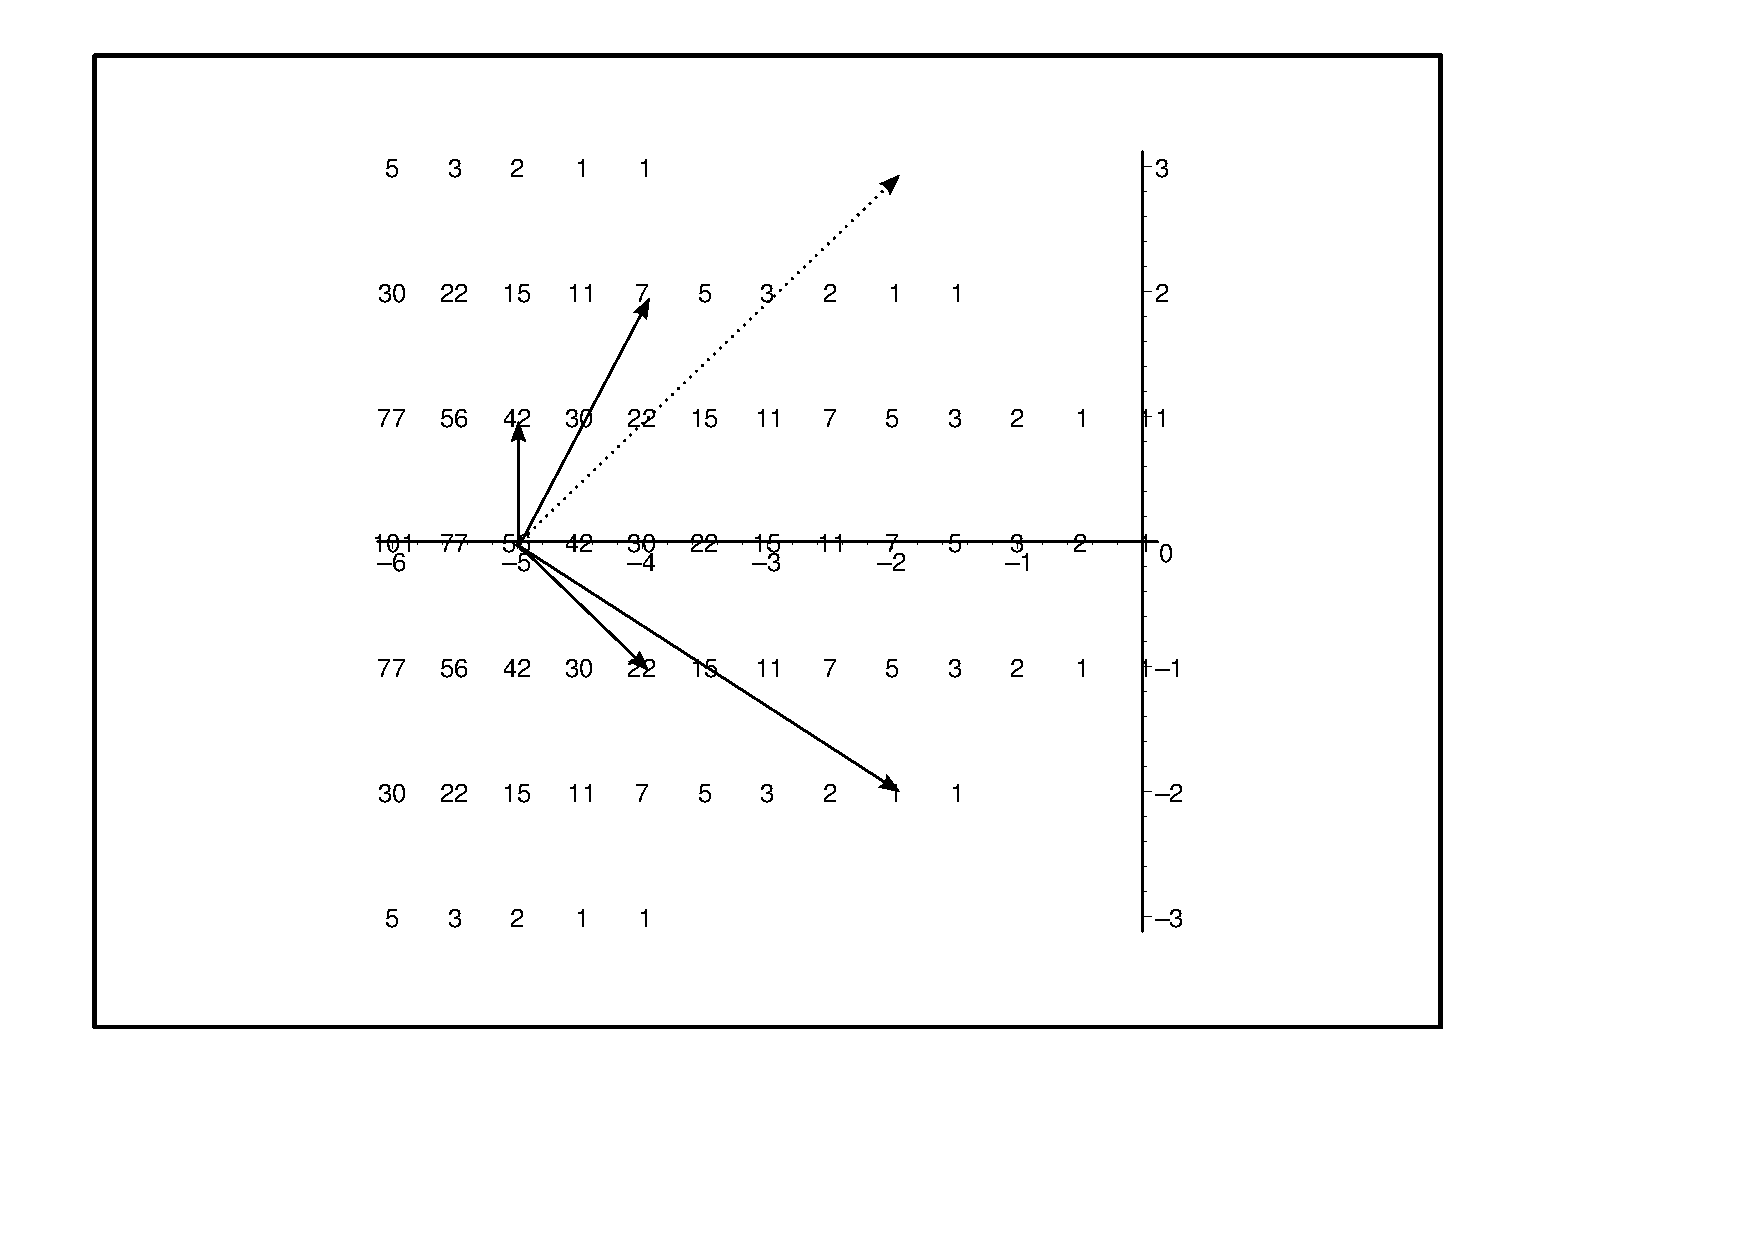
\includegraphics[width=150mm]{A1_with_star.pdf}
  }
  \caption{Computation of weight multiplicities of level 1
    representation of algebra $A_1$}
  \label{A1 with star}
\end{figure}

Weyl group of affine Lie algebra is richer than that of simple
finite-dimensional Lie algebra. It can be presented as semi-direct
product of finite Weyl group $W_0$ of simple Lie algebra
$\frak{g}_0\subset \frak{g}$ with infinite abelian group translations
along the roots of $\frak{g}_0$ which are non-imaginary roots of $\frak{g}$: 
$W=W_0\ltimes T$.

The Weyl group orbit of highest root bounds the weights with non-zero
multiplicity.

Rich Weyl symmetry of affine Lie algebras allows further improvement
of algorithm.

It can be shown that it is enough to compute multiplicities of the
weights of the form $\lambda=(\overset{\circ }{\lambda},k,n)$ where
$\overset{\circ }{\lambda}$ is finite part, $k$ - level of the
representation and $n$ - grade only for finite number of
$\overset{\circ}{\lambda}$ lying in the intersection of main Weyl
chamber with the subspace of grade zero.
Multiplicities of all other weights could be obtained by Weyl group
action. 

So all the required information can be encoded in the form of string functions:
\begin{equation}
  \label{eq:3}
  \sigma^{\mu}_{\lambda}=\sum_{k=0}^{\infty} mult(\mu-kd)q^k
\end{equation}
Where $d$ is the element dual to imaginary root $\delta$. 

It is possible to ``fold'' the star, so that the summation in formula
(\ref{eq:2}) involves only weights from main Weyl chamber. Also this
computation can be rewritten as infinite set of equations on string
functions coefficient, which can be solved recursively. See
\cite{kulish4sfa} for details.

This method is theoretically more efficient than the use of Freudenthal
formula (\ref{eq:1}) \cite{Nazarov2008}, but our implementation is
rather inefficient. Also we don't have independent realisation of algorithms,
based on (\ref{eq:1}) for affine Lie algebras, so we haven't done any
practical speed comparisons yet.
\section{Branching rules}
\label{sec:branching-rules}

Say we want to obtain decomposition of module $L^{\mu}$ of algebra
$\frak{g}$ into modules of sub-algebra $\frak{a}$
\begin{equation}
  \label{eq:4}
  L_{\frak{g}\downarrow \frak{a}}^{\mu }=\bigoplus\limits_{\nu \in P_{\frak{a}%
    }^{+}}b_{\nu }^{\left( \mu \right) }L_{\frak{a}}^{\nu }
\end{equation}
Here $\nu$ goes through weight lattice of $\frak{a}$. 

Branching coefficients can be computed in similar way using formula
(\ref{recurrent-relation}). 


Notice that to obtain the branching
rules we need only the projected singular element $\pi _{\frak{a}}\circ \Psi
^{\left( \mu\right) }$ of this module 
and the fan $\Gamma
_{\frak{a}\subset \frak{g}}$ and do not need any other properties of the module itself. 

Singular element can be computed the same way as the set of ``anomalous''
weights in section \ref{sec:representations} and then projected onto
the weight lattice of $\frak{a}$. 

The fan $\Gamma_{\frak{a}\subset \frak{g}}$ is computed as the
combination of projection of positive roots $\Delta^{+}$ of algebra
$\frak{g}$ using formula:

\begin{equation}
  \label{phi-d}
  \Phi _{\frak{a}\subset \frak{g}}=\left\{ \gamma \in P_{\frak{a}}\mid s\left(
      \gamma \right) \neq 0\right\} ;  
\end{equation}
\begin{equation}
  \label{fan-d}
  \prod_{\alpha \in \left( \pi _{\frak{a}}\circ \Delta ^{+}\right) }\left(
    1-e^{-\alpha }\right) ^{\mathrm{{mult}\left( \alpha \right) -{mult}}_{\frak{a%
      }}\mathrm{\left( \alpha \right) }}=-\sum_{\gamma \in \Phi _{\frak{a}\subset 
      \frak{g}}}s\left( \gamma \right) e^{-\gamma }.  
\end{equation}
\begin{equation}
  \label{fan-defined}
  \Gamma _{\frak{a}\subset \frak{g}}=\left\{ \xi -\gamma _{0}|\xi \in \Phi _{%
      \frak{a}\subset \frak{g}}\right\} \setminus \left\{ 0\right\} .
\end{equation}

Then branching coefficients are computed recursively using formula
(\ref{recurrent-relation}), which gives anomalous branching
coefficients which are equal to usual branching coefficients for
weights from main Weyl chamber. 

\subsection{Folding}
\label{sec:folding}

To facilitate computation of branching coefficients we can use the
idea similar to one used for computation of weight multiplicities.
There we were able to fold the star so that all the recurrent
computation took place in main Weyl chamber. 

We use the formula (\ref{eq:2}). The summation in the first term of
right-hand side goes through the set of weights $\{\xi+\pi-\omega
\rho\;|\;\omega\in W\backslash e\}$.
But for each weight $\zeta$ outside the main Weyl chamber there exists
weight $\zeta_0$ in main Weyl chamber and $\omega\in W$ such that
$\zeta=\omega \zeta_0$. So to calculate the multiplicity of $\xi$ we
sum over the set of weights inside the main Weyl chamber.

The question is if it is possible to introduce the same procedure for
computation of branching coefficients. 


\section{Details of implementation}
\label{sec:details-implementation}

The algorithms are implemented as Maple programs. Since theory of
affine Lie algebras is based upon the theory of simple
finite-dimensional Lie algebras we use Coxeter/Weyl package
\cite{stembridge1995mps} as the foundation of our work.

This design choice imposed some performance constraints but allowed us
to keep the code concise by the lack of need of reimplementation of
algorithms for computation of roots, weights and finite Weyl
reflection. So there is less than 1000 lines of code in our package.

Currently implementation allows to calculate roots, dominant weights,
weight multiplicities and branching coefficients for non-twisted
affine Lie algebras of series $A,B,C,D$ and for twisted algebras of
series $A^{(2)}$ and $D^{(2)}$.

Our program can be freely downloaded from \url{http://anton.nazarov.name/affine}

\section{Applications}
\label{sec:applications}

Weight multiplicities, calculated with presented algorithms can be
used for explicit construction of irreducible highest-weight modules.
For example, let's consider $A_3$-module of level 2 with highest
weight $\alpha_1+\alpha_2+\alpha_3$. 

String function coefficients are equal to
\begin{verbatim}
> al:=algebra_roots(A3);
              al := [e2 - e1, e3 - e2, e4 - e3, delta + e1 - e4]

> mu:=2*lambda0+sum(al[i],i=1..3);
                          mu := -e1 + e4 + 2 lambda0

> string_function(mu,mu,A3,30);
[1, 7, 32, 117, 371, 1063, 2819, 7029, 16660, 37836, 82836, 175658, 362153,

    728159, 1431447, 2757188, 5212989, 9689739, 17730751, 31977358, 56899365,

    99981354, 173632536, 298236157, 506980545, 853456334, 1423520148,

    2353697410, 3859547524, 6279119909, 10139144298]
\end{verbatim}

Weight multiplicities can be used to calculate fusion coefficients of
Wess-Zumino-Witten models, which are critical for computation of
multipoint correlation functions that determine physical quantities. 

In the paper \cite{Walton:1999xc} following equation for fusion
coefficient is derived.
\begin{equation}
  \label{eq:5}
\Nk_{\la,\mu}^\nu\ =\ \sum_{w\in W}\, (\det\,w)\, 
\mult(\mu; w\nu-\la)\ .
 \end{equation}
Here $\mult(\mu; w\nu-\la)$ denotes multiplicity of weight
$w\nu-\lambda$ in the module with highest weight $\mu$.

Branching coefficients of affine Lie algebras are used
crucial for coset construction of new models from WZW-models (see
chapter 18 in \cite{difrancesco1997cft} for details). 

Although the task of computation of branching coefficients by hand is
tedious, it is easily done by the computer.

For example, for branching of module $L^{[1,0,0]}$ of $A_2$ ($sl_3$
for complex algebras and $su_3$ for real) to sub-algebra $A_1$ ($sl_2$
or $su_2$) we have:
\begin{verbatim}
> wg:=weights(A2);
         e2    2 e1    e3                e2     e1    2 e3
 wg := [---- - ---- + ---- + lambda0, - ---- - ---- + ---- + lambda0, lambda0]
         3      3      3                 3      3      3

> tt1:=branching_rules(wg[-1],A2,A1,{e1=alpha[1]},15);
                                  tt1 := res

> tt1[lambda0];
           2      3      4       5       6       7       8       9       10
1 + q + 2 q  + 5 q  + 7 q  + 11 q  + 17 q  + 25 q  + 36 q  + 52 q  + 72 q

            11        12        13        14        15
     + 100 q   + 139 q   + 187 q   + 251 q   + 336 q  

> tt1[lambda0+e1/2];
         2      3      4       5       6       7       8       9       10
2 q + 2 q  + 4 q  + 6 q  + 10 q  + 14 q  + 24 q  + 32 q  + 48 q  + 66 q

           11        12        13        14        15
     + 94 q   + 126 q   + 176 q   + 232 q   + 314 q  
\end{verbatim}
First several terms are in agreement with the example in section
14.7.2 of the book \cite{difrancesco1997cft}.

For branching of the same module to special sub-algebra $A_2^{(2)}$ we
get
\begin{verbatim}
> tt1:=branching_rules(wg[-1],A2,tA2,{e1=alpha[1]/2},15);
                                  tt1 := res

> tt1[lambda0];
                  4      6      8      10      12      14
             1 + q  + 2 q  + 3 q  + 4 q   + 7 q   + 8 q

> tt1[lambda0+e1/2];
                                   e1
                              res[---- + lambda0]
                                   2

> tt1[lambda0+e1];
                   3      5      7      9      11       13       15
            q + 2 q  + 2 q  + 4 q  + 5 q  + 8 q   + 11 q   + 16 q
\end{verbatim}
We see that this result is in agreement with the results from the paper \cite{ilyin812pbc}.

\section{Conclusion}
\label{sec:conclusion}
We described new algorithms for representations of affine Lie algebras
and implementation of that algorithms. 

This implementation is work in progress, current version can be
downloaded from \url{http://anton.nazarov.name/affine}.

Further study is required for better performance of implementation.
Although big performance gain can be achieved for computation of
branching coefficient using the idea similar to folding of fan
\ref{sec:representations}, used
for efficient computation of string functions coefficients.

Also some additional algorithms for physical applications can be
implemented, for example for computation of fusion coefficients of
WZW-models (\ref{eq:5}). It is important to note the existence of ``Kac''
program \cite{Fuchs:1996dd} especially designed for computations in conformal field theory
models. The possibility of interoperability with ``Kac'' program
should be studied.  

\bibliography{article}{}
\bibliographystyle{utphys}

\end{document}
